%% abtex2-modelo-artigo.tex, v-1.9.6 laurocesar
%% Copyright 2012-2016 by abnTeX2 group at http://www.abntex.net.br/ 
%%
%% This work may be distributed and/or modified under the
%% conditions of the LaTeX Project Public License, either version 1.3
%% of this license or (at your option) any later version.
%% The latest version of this license is in
%%   http://www.latex-project.org/lppl.txt
%% and version 1.3 or later is part of all distributions of LaTeX
%% version 2005/12/01 or later.
%%
%% This work has the LPPL maintenance status `maintained'.
%% 
%% The Current Maintainer of this work is the abnTeX2 team, led
%% by Lauro César Araujo. Further information are available on 
%% http://www.abntex.net.br/
%%
%% This work consists of the files abntex2-modelo-artigo.tex and
%% abntex2-modelo-references.bib
%%

% ------------------------------------------------------------------------
% ------------------------------------------------------------------------
% abnTeX2: Modelo de Artigo Acadêmico em conformidade com
% ABNT NBR 6022:2003: Informação e documentação - Artigo em publicação 
% periódica científica impressa - Apresentação
% ------------------------------------------------------------------------
% ------------------------------------------------------------------------

\documentclass[
    % -- opções da classe memoir --
    article,            % indica que é um artigo acadêmico
    11pt,               % tamanho da fonte
    oneside,            % para impressão apenas no recto. Oposto a twoside
    a4paper,            % tamanho do papel. 
    % -- opções da classe abntex2 --
    %chapter=TITLE,     % títulos de capítulos convertidos em letras maiúsculas
    %section=TITLE,     % títulos de seções convertidos em letras maiúsculas
    %subsection=TITLE,  % títulos de subseções convertidos em letras maiúsculas
    %subsubsection=TITLE % títulos de subsubseções convertidos em letras maiúsculas
    % -- opções do pacote babel --
    english,            % idioma adicional para hifenização
    brazil,             % o último idioma é o principal do documento
    sumario=tradicional,
    ]{abntex2}


% ---
% PACOTES
% ---
\usepackage[table,xcdraw]{xcolor}

% ---
% Pacotes fundamentais 
% ---
\usepackage{lmodern}            % Usa a fonte Latin Modern
\usepackage[T1]{fontenc}        % Selecao de codigos de fonte.
\usepackage[utf8]{inputenc}     % Codificacao do documento (conversão automática dos acentos)
\usepackage{indentfirst}        % Indenta o primeiro parágrafo de cada seção.
\usepackage{nomencl}            % Lista de simbolos
\usepackage{color}              % Controle das cores
\usepackage{graphicx}           % Inclusão de gráficos
\usepackage{microtype}          % para melhorias de justificação
% ---
        
% ---
% Pacotes adicionais, usados apenas no âmbito do Modelo Canônico do abnteX2
% ---
\usepackage{lipsum}             % para geração de dummy text
\usepackage{fancyvrb}
\usepackage{todonotes}
\usepackage{float}
\usepackage{listings}
% ---
        
% ---
% Pacotes de citações
% ---
\usepackage[brazilian,hyperpageref]{backref}     % Paginas com as citações na bibl
\usepackage[alf]{abntex2cite}   % Citações padrão ABNT
% ---

% ---
% Configurações do pacote backref
% Usado sem a opção hyperpageref de backref
\renewcommand{\backrefpagesname}{Citado na(s) página(s):~}
% Texto padrão antes do número das páginas
\renewcommand{\backref}{}
% Define os textos da citação
\renewcommand*{\backrefalt}[4]{
    \ifcase #1 %
        Nenhuma citação no texto.%
    \or
        Citado na página #2.%
    \else
        Citado #1 vezes nas páginas #2.%
    \fi}%
% ---

% ---
% Informações de dados para CAPA e FOLHA DE ROSTO
% ---
\titulo{INE5644 - Data Mining\\ 
        Exercício Clustering}
\autor{Bruno Marques do Nascimento\thanks{brunomn95@gmail.com \hspace{1mm} - \hspace{1mm} Universidade Federal de Santa Catarina}}
\instituicao{Universidade Federal de Santa Catarina}
\local{Florianópolis - SC, Brasil}
\data{30 de Abril de 2018}
% ---

% ---
% Configurações de aparência do PDF final

% alterando o aspecto da cor azul
\definecolor{blue}{RGB}{41,5,195}

% informações do PDF
\makeatletter
\hypersetup{
        %pagebackref=true,
        pdftitle={\@title}, 
        pdfauthor={\@author},
        pdfsubject={Modelo de artigo científico com abnTeX2},
        pdfcreator={LaTeX with abnTeX2},
        pdfkeywords={abnt}{latex}{abntex}{abntex2}{atigo científico}, 
        colorlinks=true,            % false: boxed links; true: colored links
        linkcolor=blue,             % color of internal links
        citecolor=blue,             % color of links to bibliography
        filecolor=magenta,              % color of file links
        urlcolor=blue,
        bookmarksdepth=4
}
\makeatother
% --- 

% ---
% compila o indice
% ---
\makeindex
% ---

% ---
% Altera as margens padrões
% ---
\setlrmarginsandblock{3cm}{3cm}{*}
\setulmarginsandblock{3cm}{3cm}{*}
\checkandfixthelayout
% ---

% --- 
% Espaçamentos entre linhas e parágrafos 
% --- 

% O tamanho do parágrafo é dado por:
\setlength{\parindent}{1.3cm}

% Controle do espaçamento entre um parágrafo e outro:
\setlength{\parskip}{0.2cm}  % tente também \onelineskip

% Espaçamento simples
\SingleSpacing

% ----
% Início do documento
% ----
\begin{document}

% Seleciona o idioma do documento (conforme pacotes do babel)
%\selectlanguage{english}
\selectlanguage{brazil}

% Retira espaço extra obsoleto entre as frases.
\frenchspacing 

% ----------------------------------------------------------
% ELEMENTOS PRÉ-TEXTUAIS
% ----------------------------------------------------------

%---
%
% Se desejar escrever o artigo em duas colunas, descomente a linha abaixo
% e a linha com o texto ``FIM DE ARTIGO EM DUAS COLUNAS''.
% \twocolumn[           % INICIO DE ARTIGO EM DUAS COLUNAS
%
%---
% página de titulo

\maketitle


% ----------------------------------------------------------
% ELEMENTOS TEXTUAIS
% ----------------------------------------------------------
\textual

% ----------------------------------------------------------
% Introdução
% ----------------------------------------------------------
% \section*{Introdução}
% \addcontentsline{toc}{section}{Introdução}

\section*{\textbf{Respostas:}}
\addcontentsline{toc}{section}{Questões e respostas:}


% ----------------------------------------------------------
% Questão 2
% ----------------------------------------------------------
\subsection*{\textbf{Exercício 2:}}
\addcontentsline{toc}{subsection}{Exercício 3}

\begin{itemize}
    \item \textbf{ID3:}
    \begin{itemize}
        \item Tempo de construção: \textbf{0 segundos.}
        \item Características:
        \begin{itemize}
            \item Altura: 3
            \item Nodos por nível:
                \begin{itemize}
                    \item Nível 1: \textbf{1 nodo.}
                    \item Nível 2: \textbf{3 nodos.}
                    \item Nível 3: \textbf{4 nodos.}
                    \item Nível 4: \textbf{2 nodos.}
                \end{itemize}
        \end{itemize}
        \item ``Output Weka'' do algoritmo:
    \end{itemize}   

\begin{Verbatim}[frame=single, fontsize=\tiny]
=== Run information ===

Scheme:       weka.classifiers.trees.Id3 
Relation:     cogumelos.venenosos
Instances:    16
Attributes:   5
              Cor
              Altura
              Faixas
              Textura
              Venenoso
Test mode:    10-fold cross-validation

=== Classifier model (full training set) ===

Id3

Cor = Purpura
|  Faixas = Sim: Sim
|  Faixas = Nao
|  |  Altura = Alta: Nao
|  |  Altura = Baixa: Sim
Cor = Vermelha: Nao
Cor = Azul
|  Faixas = Sim: Sim
|  Faixas = Nao: Nao

Time taken to build model: 0 seconds

=== Stratified cross-validation ===
=== Summary ===

Correctly Classified Instances          13               81.25   %
Incorrectly Classified Instances         3               18.75   %
Kappa statistic                          0.625 
Mean absolute error                      0.1875
Root mean squared error                  0.433 
Relative absolute error                 36.9565 %
Root relative squared error             85.3206 %
Total Number of Instances               16     

=== Detailed Accuracy By Class ===

                 TP Rate  FP Rate  Precision  Recall   F-Measure  MCC      ROC Area  PRC Area  Class
                 0,625    0,000    1,000      0,625    0,769      0,674    0,813     0,813     Sim
                 1,000    0,375    0,727      1,000    0,842      0,674    0,813     0,727     Nao
Weighted Avg.    0,813    0,188    0,864      0,813    0,806      0,674    0,813     0,770     

=== Confusion Matrix ===

 a b   <-- classified as
 5 3 | a = Sim
 0 8 | b = Nao
\end{Verbatim}


    \item \textbf{J48 - Unpruned:}
    \begin{itemize}
        \item Tempo de construção: \textbf{0 segundos.}
        \item Características:
        \begin{itemize}
            \item Altura: 2
            \item Nodos por nível:
                \begin{itemize}
                    \item Nível 1: \textbf{1 nodo.}
                    \item Nível 2: \textbf{2 nodos.}
                    \item Nível 3: \textbf{3 nodos.}
                \end{itemize}
        \end{itemize}
        \item ``Output Weka'' do algoritmo:
    \end{itemize}   


\begin{Verbatim}[frame=single, fontsize=\tiny]
=== Run information ===

Scheme:       weka.classifiers.trees.J48 -U -M 2
Relation:     cogumelos.venenosos
Instances:    16
Attributes:   5
              Cor
              Altura
              Faixas
              Textura
              Venenoso
Test mode:    10-fold cross-validation

=== Classifier model (full training set) ===

J48 unpruned tree
------------------

Faixas = Sim
|   Cor = Purpura: Sim (3.0)
|   Cor = Vermelha: Nao (2.0)
|   Cor = Azul: Sim (4.0)
Faixas = Nao: Nao (7.0/1.0)

Number of Leaves  :     4

Size of the tree :  6


Time taken to build model: 0 seconds

=== Stratified cross-validation ===
=== Summary ===

Correctly Classified Instances          15               93.75   %
Incorrectly Classified Instances         1                6.25   %
Kappa statistic                          0.875 
Mean absolute error                      0.1146
Root mean squared error                  0.2668
Relative absolute error                 22.5845 %
Root relative squared error             52.5695 %
Total Number of Instances               16     

=== Detailed Accuracy By Class ===

                 TP Rate  FP Rate  Precision  Recall   F-Measure  MCC      ROC Area  PRC Area  Class
                 0,875    0,000    1,000      0,875    0,933      0,882    0,898     0,938     Sim
                 1,000    0,125    0,889      1,000    0,941      0,882    0,898     0,837     Nao
Weighted Avg.    0,938    0,063    0,944      0,938    0,937      0,882    0,898     0,887     

=== Confusion Matrix ===

 a b   <-- classified as
 7 1 | a = Sim
 0 8 | b = Nao
\end{Verbatim}

\begin{minipage}{\linewidth}
    \centering
    \begin{figure}[H]
        \label{j48-decision-tree}
        \caption{Árvore de decisão - J48}
        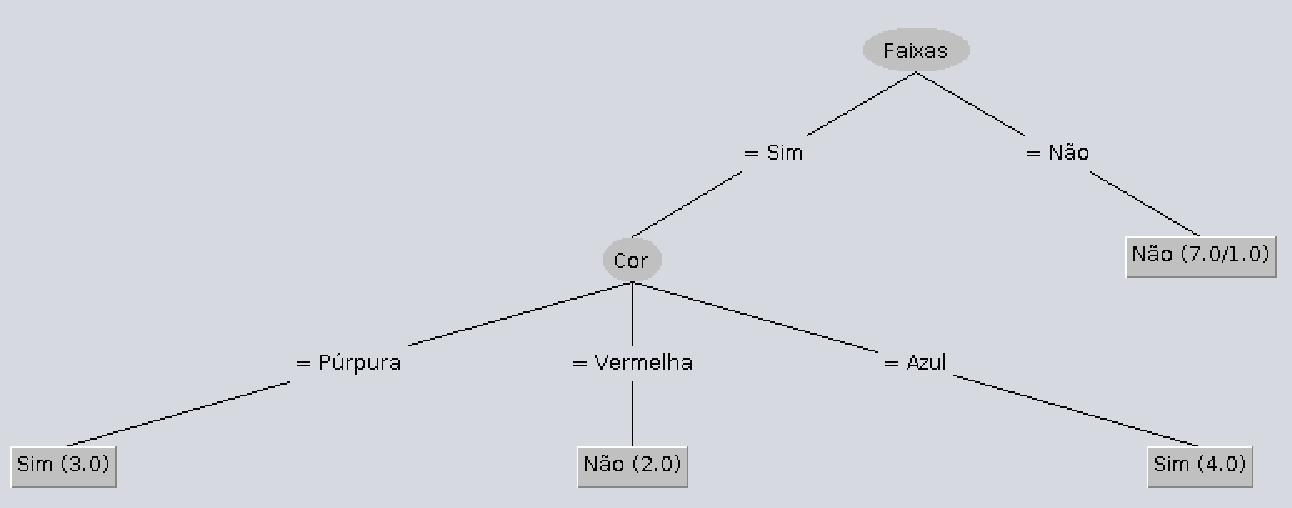
\includegraphics[width=\textwidth]{imgs/exer2-j48-tree.pdf}
    \end{figure}
\end{minipage}

\end{itemize}



% Finaliza a parte no bookmark do PDF, para que se inicie o bookmark na raiz
% ---
\bookmarksetup{startatroot}% 
% ---

% ---
% Conclusão
% ---
% \section*{Considerações finais}
% \addcontentsline{toc}{section}{Considerações finais}

% ----------------------------------------------------------
% ELEMENTOS PÓS-TEXTUAIS
% ----------------------------------------------------------
\postextual

% ----------------------------------------------------------
% Referências bibliográficas
% ----------------------------------------------------------
\nocite{material_aula}
\nocite{Witten:2016:DMF:3086818}
\bibliography{bibliography}

\end{document}